\documentclass[9pt,twocolumn,twoside]{../../styles/osajnl}
\usepackage{fancyvrb}
\journal{i524} 

\title{File Transfer Protocol - An Overview}

\author[1,*]{Sriram Sitharaman}

\affil[1]{School of Informatics and Computing, Bloomington, IN 47408, U.S.A.}

\affil[*]{Corresponding authors: srirsith@iu.edu}

\dates{\today}

\ociscodes{Cloud, I524, FTP, FTP Client, Comparison, Architecture}

% replace this with your url in github/gitlab
\doi{\url{https://github.com/cloudmesh/classes/blob/master/docs/source/format/report/report.pdf}}


\begin{abstract}


The advent of computer systems in the later part of 20th century facilitated the increase in the digitization of documents that were in existence. In order to share those documents and files among peers situated remotely, there raised a need for a mechanism which could facilitate file sharing. File Transfer Protocol developed in the late 1970s provided an efficient and reliable mechanism for sharing files among hosts. File Transfer Protocol (FTP) and its architecture is discussed along with the alternatives to FTP and how they fare when compared to FTP. FTP clients used for managing the file transfer at the client side is also discussed.\newline
\end{abstract}

\setboolean{displaycopyright}{true}

\begin{document}

\maketitle
\tableofcontents % Print the contents section
\section{Introduction}
According to \cite{www-wiki-ftp} FTP is an acronym for File Transfer Protocol. It is network protocol standard used for transferring files between two computer systems or between a client and a server. It is a part of Application layer of the Internet Protocol Suite and works along with HTTP/SSH and follows a client-server model architecture. Secure systems asks the client to authenticate themselves using a Username and Password registered with the server to access the files via FTP. The specification for FTP was first written by  Abhay Bhushan \cite{www-rfc114} in 1971 and is termed as RFC114. The current specification, RFC959 in use was written in 1985. Several other versions of the specification are available which provides firewall friendly FTP access, additional security extensions, support for IPV6 and passive mode file access respectively. FTP can be used in command line in most of the operating systems to transfer files. There are FTP clients such as WinSCP, FileZilla etc. which provides a graphical user interface to the clients to authenticate themselves (sign on) and access the files from the server.


\section{Architecture}

\begin{figure*}[hbt]
\begin{center}
\centering
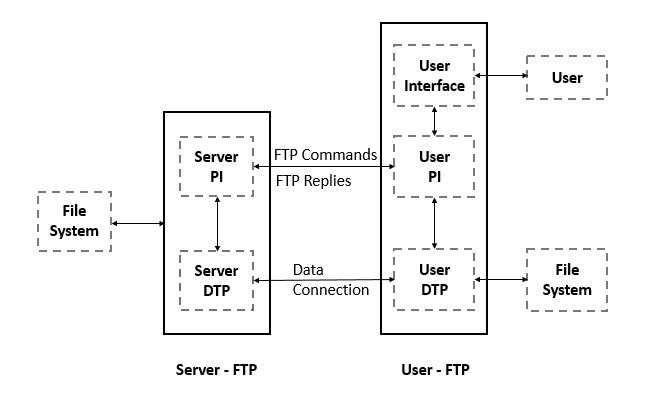
\includegraphics[width =6in ,height=3.5in]{images/Architecture}
\caption{Model for FTP usage \cite{www-rfc959}}
\label{fig:arch}
\end{center}
\end{figure*}

Figure \ref{fig:arch} shows the architecture of a model for using File Transfer Protocol. It is essential to understand the different components of the architecture to understand the flow of FTP.The next section describes in brief about the components that are part of the model architecture.

\subsection{Components in FTP model}
As shown in Figure 1., FTP model consists of two major components Server side FTP component and a client side FTP component. Each of those components consists of a Protocol Interpreter (PI) which takes of the respective protocol definitions for the user and server end, and a Data Transfer Process (DTP) which establishes and manages the connection between the server and the client. Apart from these two, client side FTP component has a User Interface through which the User authenticates himself with the server and requests for the files to be transferred.

\subsection{File System}
File system is the place where the files are located. It is present in both the client and the server end. When the user want to request a file from the server, a pathname (a character string) has to be specified as an input to the file system to locate the file. A location has be to specified by user/client in the client side for storing the file transferred by the client. 

\subsection{File Request/Receive Process}
Once the user wants to request a file from the server, the user protocol interpreter is responsible for initiating the connection process to the server-FTP. Once the control connection is established by the user PI, it generates standard FTP commands to the server. User PI is also responsible for managing the data transfer process (DTP) as part of the file transfer process. In response to the commands sent from the user, replies are sent by the server which acts as an acknowledgement.\\

\subsection{FTP Commands}
The FTP commands specifies the following parameters for the data connection:
\begin{enumerate}
    \item \textbf{Data port} - Port is a communication endpoint in an operating system \cite{www-wiki-port}. Each computer system has ports numbered from 0 to 1023 each of which can be uniquely associated with a process. For File Transfer Protocol, the designated port number is 21.
    \item \textbf{Transfer mode} - It defines the type of transfer process using which the data is sent between the client and the server. There are 3 different modes through which this can be accomplished:
    \begin{enumerate}
        \item Stream mode - It is used when transferring data continuously from one end to another.
        \item Block mode - When there is a limitation on the size of data that can be sent, data is split into blocks of size (with a threshold on size) and sent across one by one according to the order of split.
        \item Compressed mode - data is compressed using a compression algorithm and then transferred to the other system.
    \end{enumerate}
    \item \textbf{Representation type} - It defines the type of the data that is being transferred between the server to the client
    \begin{enumerate}
    \item ASCII  mode - used if the data is of textual format. 
    \item Image mode - For transferring data in binary format as bytestreams. 
    \item EBCDIC  mode - used for transferring text data between systems that follows the EBCDIC character format.
    \item Local mode - used between systems that follow similar characteristics in data format.
    \end{enumerate}
    \item \textbf{Structure} - Specifies the structure of the file that is sent across. It can be a: (1) file structure - when the data is continuous sequence of bytes, (2) record structure - when the data is a relational database table with sequential records on each line of the file and (3) page structure - when the data in each file is stored as independent indexed pages.  
    \item \textbf{Type of the file system operation} - store, retrieve, append, delete, etc.
\end{enumerate}
\begin{table*}[hbt]
\centering


\begin{tabular}{|l|l|l|l|l|l|l|l|l|l|}
\hline
\rowcolor[HTML]{D9F4F4} 
\textbf{Client} & \textbf{Creator}         & \textbf{Software license} & \textbf{Over 2GB?} & \textbf{Interface} & \textbf{Windows} & \textbf{OS X} & \textbf{Linux} & \textbf{BSD} & \textbf{Unix} \\ \hline
Cyberduck       & David V. Kocher          & GPL                       & Yes                & GUI                & Yes              & Yes           & No             & No           & No            \\ \hline
FileZilla       & Community                & GPL                       & Yes                & GUI                & Yes              & Yes           & Yes            & Yes          & Yes           \\ \hline
WinSCP          & Martin Přikryl           & GPL                       & Yes                & GUI/CLI            & Yes              & No            & No             & No           & No            \\ \hline
CuteFTP         &Globalscape & Proprietary               & Yes                & GUI                & Yes              & Yes           & No             & No           & No            \\ \hline
Classic FTP     & NCH Software             & Proprietary               & Yes                & GUI                & Yes              & Yes           & No             & No           & No            \\ \hline
\end{tabular}
\caption{Comparisons of FTP clients \cite{www-wiki-perf}}
\label{perf}
\end{table*}

\begin{table*}[hbt]
\centering
\begin{tabular}{|l|l|l|l|l|l|l|l|}
\hline
\rowcolor[HTML]{EFEFEF} 
\textbf{Client}      & \textbf{FTP} & \textbf{FTP over SSH} & \textbf{SFTP} & \textbf{Compression} & \textbf{\begin{tabular}[c]{@{}l@{}}Remote\\   Compression\end{tabular}} & \textbf{Resume Download} & \textbf{Passive mode} \\ \hline
\textbf{Cyberduck}   & Yes          & No                    & Yes           & No                   & Yes                                                          & Yes                      & Yes                   \\ \hline
\textbf{FileZilla}   & Yes          & Yes                   & Yes           & No                   & No                                                                      & Yes                      & Yes                   \\ \hline
\textbf{WinSCP}      & Yes          & Yes                   & Yes           & Yes      & Yes                                                      & Yes                      & Yes                   \\ \hline
\textbf{CuteFTP}     & Yes          & Yes                   & Yes           & Yes                  & No                                                                      & Yes                      & Yes                   \\ \hline
\textbf{Classic FTP} & Yes          & No                    & No            & No                   & ?                                                                       & ?                        & ?                     \\ \hline
\end{tabular}
\caption{Comparison of Functionalities - FTP clients \cite{www-wiki-perf}}
\label{func}
\end{table*}

\subsection{Response from Server DTP}
The user DTP should listen on the designated port mentioned in the parameters sent during the FTP commands and the server DTP initiates the data transfer process as per the specified parameters. The end of the data transfer process is indicated by the End-of-File (EOF) sequence which indicates the end of the file being transferred. The data transfer process, in general is made through a full duplex connection. A duplex connection \cite{www-wiki-duplex} is defined as a communication channel mechanism when the systems present at either end of the channel can communicate with each other in both directions. Full duplex is when the communication from both ends can occur simultaneously.

\section{Alternatives to FTP}

After its arrival in 1971 termed under RFC114 \cite{www-rfc114}, FTP has underwent multiple revisions in its usage specification and the current one is defined under RFC959 \cite{www-rfc959}. Though FTP is the standard file transfer mechanism that can be used in building applications, it is advisable to use modified versions of FTP when it comes to enterprise level applications.

\subsection{Managed File Transfer (MFT)}

MFT \cite{www-wiki-mft} is a secured file transfer protocol used by enterprises as an alternative to FTP. Some of the key features that makes MFT better than FTP include its ability to provide high secured connectivity, reporting of status of file transfer, auditability, payload management , monitoring of performance metrics \cite{www-wiki-perf} like time and latency of file transfer etc. 


\subsection{Trivial File Transfer Protocol (TFTP)}

TFTP \cite{www-wiki-tftp} is a type of file transfer protocol which the transfer of files between a system and multiple remote systems in parallel. It is mainly used for booting of systems remotely from a local area network.

\subsection{Simple File Transfer Protocol (SFTP)}

Simple File Transfer Protocol (SFTP) \cite{www-wiki-ftp} (not to be confused with Secure Shell File Transfer Protocol) is a unsecured file transfer protocol with complexity between FTP and TFTP. On account of it being a simple protocol, it's command set comprises of only 11 commands. It is also known for supporting login with user id and password.

\subsection{Secure Shell File Transfer Protocol (SFTP)}
SSH File Transfer Protocol (SSH FTP or SFTP) \cite{www-wiki-sftp} is a file transfer mechanism that offers the same set of commands and functions as FTP but enables the data transfer with a secured shell connection. SSH is a encrypted network protocol for operating over an unsecured network \cite{www-wiki-ssh}. \\\\

\section{Customized File Transfer Protocol (FTP) mechanisms}
McWilliams in his patent \cite{mcwilliams2001high} proposed a modified version of file transfer protocol which provides the advantages that the files are transferred at a time specified by the client and that only those files which have been selected by the client are transferred. Bahlmann et.al  has specified an on the fly version of FTP \cite{bahlmann2001fly} which enables the creation of files on the fly based on the parameters sent through the FTP connection.

\section{FTP clients}
An FTP client is a software which uses the FTP protocol to transfer files to and from a remote computer. FTP clients provide a Command Line Interface (CLI) or a Graphical User Interface (GUI) for the user to authenticate themselves with the server and request for file transfer.
\subsection{Comparison of FTP Clients}
As mentioned in the previous section, FTP client assists the user in the process of file transfer from the client. There are several FTP clients available in the market, open source as well as proprietary. Table \ref{perf} and Table \ref{func} shows the five selected FTP clients and the characteristics of them with respect to file transfer \cite{www-wiki-ftpclientcomp}.

One of the important feature any FTP client is it's ability to transfer large files. According to \cite{www-wiki-ftpclientcomp}, the five clients listed here as well most of the ftp clients available in the market supports large file transfer. And the next important factor is the ftp client's ability to incorporate different file transfer mechanisms. While it is clear from the Table \ref{func} that all of the clients supports FTP, the basic transfer mechanism. According to \cite{www-wiki-ftpclientcomp}, FTP is supported by almost all of clients available, while SSH FTP is supported only by a few. Since a secured shell connection for data transfer is required to support SSH FTP, it is understandable that most of these versions of ftp clients are sticking to the standard file transfer mechanisms. Table 2 also points out characteristics like if data compression is allowed (at both ends), if resume option is available for file transfer, and if passive mode (when the client is protected by a firewall) option is available. \cite{www-wiki-ftpclientcomp} lists several other ftp clients open source and proprietary and the characteristics of them.

\section{Conclusion}

A brief introduction was given to File transfer protocol and its architecture which gives a clear picture of the flow involved in the file transfer process between a client and a server. Parameters involved in the FTP command from the client to the server, and the range of values it can take depending on the use case was explained. Different alternatives to FTP was put forth, and how each of them differs and performs when compared to FTP is discussed. Finally, the notion of FTP client is introduced and FTP clients were compared across different parameters.

\bibliography{references}

\end{document}
